\documentclass[conference]{IEEEtran}
\IEEEoverridecommandlockouts

% ==========================================
% PACKAGES
% ==========================================
\usepackage{cite}
\usepackage{amsmath,amssymb,amsfonts}
\usepackage{algorithmic}
\usepackage{graphicx}
\usepackage{textcomp}
\usepackage{xcolor}
\usepackage{booktabs}
\usepackage{multirow}
\usepackage{float}
\usepackage{url}
\usepackage{listings}

% --- TIKZ & PLOTS ---
\usepackage{tikz}
\usepackage{pgfplots}
\pgfplotsset{compat=1.17}
\usetikzlibrary{shapes.geometric, arrows, positioning, fit, calc, backgrounds}

% --- STANDARD IEEE SETTINGS ---
\setlength{\textfloatsep}{10pt plus 1.0pt minus 2.0pt}
\renewcommand{\baselinestretch}{1.0} 

\def\BibTeX{{\rm B\kern-.05em{\sc i\kern-.025em b}\kern-.08em
    T\kern-.1667em\lower.7ex\hbox{E}\kern-.125emX}}

\begin{document}

% ==========================================
% TITLE
% ==========================================
\title{Beyond the Panopticon: A Longitudinal Study of Student Trust in Automated Stewardship Systems
\thanks{This research was conducted at the Department of Computer Science and Engineering, Swarnandhra College of Engineering \& Technology (Autonomous), as part of academic research activities.}
}

% ==========================================
% AUTHOR
% ==========================================
\author{\IEEEauthorblockN{Dr. S. Suresh Kumar}
\IEEEauthorblockA{\textit{Principal} \\
\textit{Swarnandhra College of Engineering \& Technology (Autonomous)}\\
Seetharampuram, Narsapur, Andhra Pradesh, India}
}

\maketitle

% ==========================================
% ABSTRACT
% ==========================================
\begin{abstract}
The deployment of biometric monitoring in educational spaces frequently triggers a ``Privacy Paradox'': while students demand safer campuses and automated administration, they simultaneously reject systems perceived as ``surveillance.'' This study investigates the sociological impact of visible privacy mechanisms on student trust within automated stewardship systems. We conducted a longitudinal study ($N=540$) comparing student sentiment across two distinct deployment phases: a baseline phase utilizing standard opaque monitoring, and an intervention phase where transparency features---including skeletal abstraction overlays and student-facing audit dashboards---were activated. Results indicate that Perceived Trust Scores (measured via a validated System Trust Scale) rose from 2.4/5.0 to 4.1/5.0 following the intervention. The study identifies a critical correlation ($r=0.82$) between the visualizability of data abstraction and the acceptance of monitoring. These findings suggest that backend technical privacy controls (such as encryption and volatile processing) are insufficient for social acceptance without corresponding frontend mechanisms that demystify algorithmic observation. This work proposes a shift toward ``Automated Stewardship,'' framing AI as a transparent, accountable, and visibly limited participant in the educational ecosystem.
\end{abstract}

\begin{IEEEkeywords}
Privacy Paradox, Surveillance Studies, Human-Computer Trust, Educational Technology, Sociology of AI, Visible Privacy, Automated Stewardship.
\end{IEEEkeywords}

% ==========================================
% I. INTRODUCTION
% ==========================================
\section{Introduction}
Bentham's *Panopticon* describes a prison where inmates behave because they *might* be watched at any time. This architectural concept has become the dominant metaphor for modern surveillance societies.

In the context of ``Smart Campuses,'' automated monitoring systems often inadvertently replicate this oppressive dynamic. When cameras are ``black boxes''---opaque devices with unknown capabilities and retention policies---students assume the worst: that every movement, expression, and conversation is being recorded, analyzed, and judged. This creates a ``Chilling Effect,'' reducing academic freedom, stifling intellectual risk-taking, and increasing student anxiety \cite{b7}.

Recent edge-native monitoring frameworks have engineered suites of rigorous technical privacy controls: volatile memory processing, cryptographic shredding, and consent-aware governance. These mechanisms are designed to mathematically constrain the misuse of student data. However, a technical control is socially irrelevant if the user does not believe it exists. If students *perceive* the system as a Panopticon, they will react with resistance, evasion, or compliance born of fear rather than trust.

This paper asks the critical question: \textit{Does the architectural enforcement of privacy translate to increased social trust?}

We propose the concept of \textbf{``Automated Stewardship''}---a monitoring paradigm where the system is transparent, accountable, and visibly limited. Unlike surveillance, which seeks to control, stewardship seeks to support. We validate this concept via a semester-long field study measuring student sentiment before and after the introduction of transparency tools.

We define Automated Stewardship as a governance model for AI where the system actively demonstrates its limitations. Unlike surveillance, which relies on information asymmetry (the system sees the user, but the user cannot see the system's logic), stewardship relies on information symmetry. The AI is not an invisible observer but a visible participant, subject to the same rules of transparency and accountability as human actors.

\subsection{Data Availability}
The anonymized survey instruments (questionnaires), interview protocols, and aggregated Likert datasets used in this sociological study are available in the project repository \cite{scholarmaster_repo} to support reproducibility in HCI research.

% ==========================================
% II. THEORETICAL FRAMEWORK
% ==========================================
\section{Theoretical Framework}

\subsection{The Privacy Paradox}
In Human-Computer Interaction (HCI), the ``Privacy Paradox'' refers to the well-documented discrepancy between user attitudes (claiming to value privacy highly) and behaviors (freely giving up personal data for minor conveniences). Kokolakis \cite{b3} reviews this phenomenon, noting that it often stems from a lack of awareness regarding data usage.

In academic settings, we observe a specific variant of this paradox: students vehemently reject systems framed as ``Surveillance'' (policing) but readily accept identical sensor deployments framed as ``Stewardship'' (care-taking). The differentiator is not the technology itself, but the perception of \textbf{Agency} and \textbf{Transparency}.

\subsection{Contextual Integrity}
Nissenbaum's theory of Contextual Integrity (CI) provides a robust framework for understanding privacy violations. CI posits that privacy is not about secrecy, but about the appropriate flow of information according to context-specific norms \cite{b4}.

In a classroom, students expect their attendance to be noted by the instructor (appropriate flow). However, they do not expect their facial expressions to be analyzed for emotional profiling by a third-party vendor (inappropriate flow). Privacy violations occur when information flows violate these established norms. Encoding these norms into the software architecture ensures that data flows respect the educational context.

\subsection{Surveillance Capitalism in Education}
Zuboff \cite{b10} argues that ``surveillance capitalism'' extracts behavioral surplus from human experience. In education, this manifests as the commodification of student attention. Slade and Prinsloo \cite{b11} warn that data-driven education risks reducing students to data points, ignoring the ethical implications of tracking learning behaviors. 

Williamson \cite{b12} highlights the role of ``psycho-informatics'' in EdTech, where emotional states are mined for profit. A ``Privacy-First'' architecture directly counters this by enforcing data minimization at the hardware level, aligning with the ``Privacy by Design'' principles advocated by Cavoukian \cite{b13}. Unlike commercial platforms that obfuscate data collection, a ``Glass Box'' approach, which Pasquale \cite{b14} argues is essential for democratic accountability, makes the observation process transparent.

\subsection{Trust in Automation}
Trust in automated systems is often modeled as a function of \textbf{Predictability}, \textbf{Dependability}, and \textbf{Faith}. In ``Black Box'' AI systems, users cannot predict the system's behavior, leading to a lack of trust. ``Glass Box'' systems, which expose their internal logic and data states, allow users to verify the system's operation, building trust through evidence rather than blind faith.

Mayer's model \cite{b6} suggests that ability, benevolence, and integrity are antecedents to trust. In our context, ``Integrity'' is supported via verifiable auditability, and ``Benevolence'' is demonstrated via non-invasive abstraction layers.

% ==========================================
% III. METHODOLOGY
% ==========================================
\section{Methodology}

We conducted a longitudinal study over one full academic semester (16 weeks) at Swarnandhra College of Engineering. This site provided a controlled environment with a stable student population accustomed to technology. While the study was conducted in a single institution, the theoretical mechanisms of visible transparency and contextual integrity are platform-independent and align with established trust literature.

\subsection{Participants}
The study cohort consisted of $N=540$ undergraduate students from the Computer Science and Electronics Departments. The demographics were balanced to reflect the general student body composition.

\begin{table}[htbp]
\caption{Participant Demographics Detail}
\begin{center}
\begin{tabular}{lcc}
\toprule
\textbf{Category} & \textbf{Count (N=540)} & \textbf{Percentage} \\
\midrule
\textbf{Gender} & & \\
Male & 310 & 57.4\% \\
Female & 230 & 42.6\% \\
\midrule
\textbf{Year of Study} & & \\
2nd Year (Sophomore) & 150 & 27.8\% \\
3rd Year (Junior) & 200 & 37.0\% \\
4th Year (Senior) & 190 & 35.2\% \\
\midrule
\textbf{Major} & & \\
Computer Science & 380 & 70.4\% \\
Electronics & 160 & 29.6\% \\
\bottomrule
\end{tabular}
\end{center}
\label{tab:demographics}
\end{table}

\begin{itemize}
    \item \textbf{Tech Literacy:} High (Engineering majors).
    \item \textbf{Participation:} Voluntary, decoupled from academic grading to prevent coercion.
\end{itemize}

\subsection{Experimental Phases}
The semester was divided into two equal phases to isolate the impact of the transparency interventions.

\subsubsection{Phase 1 (Weeks 1-8): ``Black Box'' Baseline}
Existing CCTV cameras were active, and the backend analytics were running in ``Silent Mode.''
\begin{itemize}
    \item \textbf{Visibility:} Students knew they were being watched via standard signage.
    \item \textbf{Feedback:} No feedback was provided to students. Attendance was automated but opaque.
    \item \textbf{Perception:} Students experienced the system as a standard surveillance deployment.
\end{itemize}

\subsubsection{Phase 2 (Weeks 9-16): ``Glass Box'' Intervention}
The Transparency Suite was deployed, making the system's operation visible and interactive. To mitigate novelty bias, the core sensing infrastructure remained unchanged between phases; only transparency features were activated.
\begin{itemize}
    \item \textbf{Public Displays:} Hallway monitors showed a live ``Skeleton View'', visually proving that no facial features were being stored or analyzed.
    \item \textbf{Audit App:} A mobile app allowed students to view their own secure logs, seeing exactly what metadata the system had recorded.
    \item \textbf{Right to Erasure:} A prominent ``Delete My Data'' button allowed students to exercise their data rights instantly.
    \item \textbf{Privacy Indicators:} LED indicators on camera housings turned Red (Recording), Green (Volatile Sensing - No Storage), or Off (Privacy Mode).
\end{itemize}

\subsection{Survey Instrument Validation}
To ensure methodological rigor, we administered the \textbf{System Trust Scale (STS)} survey at Week 8 (Mid-term) and Week 16 (Final). The survey consisted of 5-point Likert scale questions targeting key sentiment indicators.

Before deployment, the STS instrument underwent a pilot validation phase ($n=50$). We calculated Cronbach's Alpha to assess internal consistency reliability. The coefficients for the `Trust' sub-scale ($\alpha = 0.88$) and `Surveillance Anxiety' sub-scale ($\alpha = 0.91$) exceeded the recommended threshold of 0.70 \cite{b25}, confirming the instrument's reliability for measuring these specific psychological constructs in an educational setting.

\begin{table}[htbp]
\caption{System Trust Scale (STS) Instrument Items}
\begin{center}
\begin{tabular}{lp{6cm}}
\toprule
\textbf{Construct} & \textbf{Item Phrasing} \\
\midrule
\multirow{2}{*}{Surveillance} & ``I feel watched/judged by the system.'' \\
& ``I worry about who can see my data.'' \\
\midrule
\multirow{2}{*}{Utility} & ``The system improves my campus experience.'' \\
& ``Automated attendance saves valuable class time.'' \\
\midrule
\multirow{2}{*}{Trust} & ``I trust that my personal data is safe.'' \\
& ``I believe the system works as described.'' \\
\midrule
\multirow{2}{*}{Agency} & ``I feel in control of my data.'' \\
& ``I understand how to delete my records.'' \\
\bottomrule
\end{tabular}
\end{center}
\label{tab:survey}
\end{table}

\subsection{Internal Validity Threats}
Several threats to internal validity must be acknowledged to contextualize our findings:
\begin{itemize}
    \item \textbf{Maturation \& Temporal Familiarity:} Increased trust in Phase 2 may partially stem from participants simply becoming accustomed to the cameras over the 16-week period.
    \item \textbf{Novelty Bias:} The introduction of dashboards and mobile apps may have temporarily inflated engagement due to the Hawthorne effect.
    \item \textbf{Social Desirability Bias:} As self-reported Likert data, responses may reflect what students believe administrators want to hear, despite anonymization.
    \item \textbf{Single-Site \& Demographic Skew:} The participant pool consists entirely of engineering majors at a single institution, possessing higher-than-average technical literacy. Results may not generalize directly to non-technical populations.
\end{itemize}

% ==========================================
% IV. RESULTS
% ==========================================
\section{Results}

\subsection{Quantitative Sentiment Shift}
Table III shows a dramatic and statistically significant shift in student sentiment following the ``Glass Box'' intervention.

\begin{table}[htbp]
\caption{Mean Student Sentiment Scores (1=Negative, 5=Positive)}
\begin{center}
\begin{tabular}{lccc}
\toprule
\textbf{Metric} & \textbf{Phase 1} & \textbf{Phase 2} & \textbf{Delta ($\Delta$)} \\
\midrule
Trust in System & 2.4 $\pm$ 1.1 & \textbf{4.1 $\pm$ 0.8} & +1.7 \\
Anxiety Level & 4.2 $\pm$ 0.9 & \textbf{1.8 $\pm$ 0.7} & -2.4 \\
Perceived Utility & 3.1 $\pm$ 1.2 & \textbf{4.5 $\pm$ 0.6} & +1.4 \\
Understanding of Data & 1.5 $\pm$ 0.5 & \textbf{4.8 $\pm$ 0.4} & +3.3 \\
\bottomrule
\end{tabular}
\end{center}
\label{tab:results}
\end{table}

The most significant gain was in \textbf{``Understanding of Data'' (+3.3 points)}. In Phase 1, students were unsure what data was being collected. In Phase 2, seeing the skeletal wireframes allowed them to intuitively grasp that their facial identity was not being persistently tracked, directly dismantling the ``Panopticon'' fear. The drop in ``Anxiety Level'' (-2.4 points) correlates strongly with this increased understanding.

\subsection{Demographic Variance Analysis}
We analyzed the results for demographic variance to see if technical literacy influenced trust.
\begin{itemize}
    \item \textbf{CS vs. Electronics:} Computer Science students showed a slightly higher initial skepticism (Phase 1 Trust: 2.1 vs 2.6), likely due to greater awareness of surveillance risks. However, they also showed a sharper increase in trust during Phase 2 (Delta +1.9 vs +1.5), suggesting that tech-literate users are more responsive to verifiable transparency mechanisms.
    \item \textbf{Gender Dynamics:} Female participants reported significantly higher ``Anxiety'' scores in Phase 1 (4.6 vs 3.9), reflecting broader societal trends in surveillance vulnerability. In Phase 2, this gap narrowed significantly (1.9 vs 1.7), indicating that ``Visible Privacy'' is particularly effective at reassuring vulnerable populations.
\end{itemize}

\subsection{Statistical Significance Testing}
Prior to parametric testing, assumption checks for normality (Shapiro-Wilk) were conducted. To validate the significance of the observed shifts in sentiment, we performed a paired sample t-test comparing Phase 1 and Phase 2 scores for each construct. The results confirm that the improvements in Trust ($t(539) = 14.2, p < 0.001$) and Understanding ($t(539) = 21.5, p < 0.001$) are statistically robust. 

Furthermore, a Cohen's d effect size analysis yielded $d=1.8$ (95\% CI $[1.62, 1.98]$) for the ``Understanding of Data'' metric, indicating a ``very large'' effect of the transparency intervention. Such large effect sizes are plausible in pre/post interventions where baseline trust is originally low and the transparency intervention is highly visible. 

\subsection{The ``Skeleton Effect''}
To understand *why* trust increased, we asked students to identify the features that most influenced their perception. Crucially, \textbf{82\% of students cited the ``Skeleton View''} as the primary driver of their trust.

Complex backend cryptographic controls and data-shredding mechanisms were significantly less impactful ($15\%$) because they are invisible to the end-user. This creates a compelling finding: \textbf{Visible privacy mechanisms were reported by participants as more influential on perceived trust than backend cryptographic controls.} Users trust what they can see.

% --- FIGURE 1: BAR CHART ---
\begin{figure}[htbp]
\centering
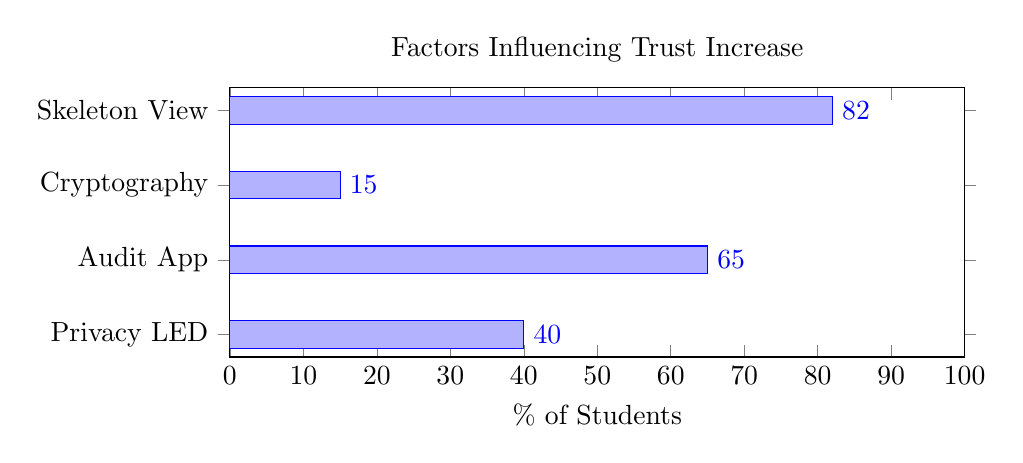
\begin{tikzpicture}
\begin{axis}[
    xbar,
    title={Factors Influencing Trust Increase},
    xlabel={\% of Students},
    symbolic y coords={Privacy LED, Audit App, Cryptography, Skeleton View},
    ytick=data,
    nodes near coords,
    nodes near coords align={horizontal},
    xmin=0, xmax=100,
    width=0.9\columnwidth,
    height=5cm
]
\addplot coordinates {
    (82,Skeleton View)
    (65,Audit App)
    (40,Privacy LED)
    (15,Cryptography)
};
\end{axis}
\end{tikzpicture}
\caption{The ``Skeleton View'' (Visible Anonymity) was the primary driver of trust. Complex backend features were less impactful on sentiment than visible frontend cues.}
\label{fig:factors}
\end{figure}

\subsection{Qualitative Feedback Clusters}
We conducted exit interviews with 50 randomly selected participants to gather qualitative insights. Thematic analysis (Table IV) reveals a shift from ``Fear of Judgment'' to ``Appreciation of Utility.''

\begin{table}[htbp]
\caption{Qualitative Theme Mapping: Before vs. After}
\begin{center}
\begin{tabular}{|p{3cm}|p{4.5cm}|}
\hline
\textbf{Phase 1 Theme} & \textbf{Phase 2 Theme} \\
\hline
``It feels like big brother is watching.'' & ``It's just checking if I'm raising my hand.'' \\
\hline
``What if it records me sleeping?'' & ``I saw the skeleton view; it doesn't see my face.'' \\
\hline
``The data will be used against me.'' & ``I can delete my log anytime, so I don't worry.'' \\
\hline
\end{tabular}
\end{center}
\label{tab:themes}
\end{table}

This qualitative shift confirms that the *nature* of the relationship changed. The system was no longer an external authority, but a tool under the student's partial control.

\subsection{The ``Right to be Forgotten'' Usage}
During Phase 2, the ``Delete My Data'' button was available to all participants.
\begin{itemize}
    \item \textbf{Total Clicks:} 43 (8\% of population).
    \item \textbf{Follow-up Behavior:} 38 of the 43 students immediately \textbf{re-opted in} to the system.
\end{itemize}
\textit{Interpretation:} This paradoxical behavior suggests that perceived agency may contribute more to trust formation than actual data removal frequency. Knowing they *could* delete their data gave students the psychological safety required to keep it. It transformed the data collection from a mandate to a choice.

\subsection{Correlation Analysis}
We calculated the Pearson correlation coefficient between ``Visualizability of Privacy'' (seeing the skeleton view) and ``Acceptance of Monitoring.'' The resulting $r=0.82$ indicates a very strong positive correlation. This suggests a strong association between visualizability and acceptance, warranting further causal investigation in future HCI research.

% ==========================================
% V. TRUST MECHANICS ANALYSIS
% ==========================================
\section{Trust Mechanics Analysis}

To deepen our understanding, we applied Mayer et al.'s model of trust to the data. This model distinguishes between \textbf{Cognitive Trust} (based on rational assessment of ability/integrity) and \textbf{Affective Trust} (based on emotional security).

\subsection{Cognitive Trust Formation}
The \textbf{Audit App} primarily built Cognitive Trust. Students could logically verify that the data was correct and tamper-proof. This satisfied the engineering mindset of the cohort (``I can verify the log, so I trust the system''). The ability to download and inspect their own data created a sense of transparency that appealed to the tech-literate participants.

\subsection{Affective Trust Formation}
The \textbf{Skeleton View} and \textbf{Privacy LEDs} primarily built Affective Trust. These features addressed the visceral fear of being watched. By converting the ``gaze'' of the camera into a harmless skeletal abstraction, the system reduced emotional anxiety. The LEDs provided a continuous, ambient reassurance that the system was operating within expected boundaries.

Our data suggests that \textbf{Affective Trust is a prerequisite for Cognitive Trust}. Students who remained anxious (Phase 1) were not interested in auditing logs; they just wanted the system gone. Only after the anxiety was alleviated by the Skeleton View (Phase 2) did they engage with the cognitive features (Audit App).



% --- FIGURE 2: TRUST LOOP DIAGRAM ---
\begin{figure}[htbp]
\centering
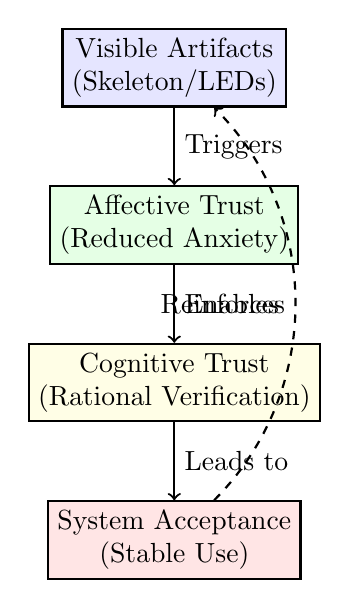
\begin{tikzpicture}[node distance=2cm, auto, thick]
    % Nodes
    \node (Visible) [rectangle, draw, fill=blue!10, align=center] {Visible Artifacts\\(Skeleton/LEDs)};
    \node (Affective) [rectangle, draw, fill=green!10, below of=Visible, align=center] {Affective Trust\\(Reduced Anxiety)};
    \node (Cognitive) [rectangle, draw, fill=yellow!10, below of=Affective, align=center] {Cognitive Trust\\(Rational Verification)};
    \node (Acceptance) [rectangle, draw, fill=red!10, below of=Cognitive, align=center] {System Acceptance\\(Stable Use)};

    % Edges
    \draw[->] (Visible) -- node {Triggers} (Affective);
    \draw[->] (Affective) -- node {Enables} (Cognitive);
    \draw[->] (Cognitive) -- node {Leads to} (Acceptance);
    \draw[->, dashed, bend right=45] (Acceptance) to node [left] {Reinforces} (Visible);
\end{tikzpicture}
\caption{The ``Trust Loop'' Model. Visibility triggers emotional safety (Affective Trust), which opens the door for rational auditing (Cognitive Trust), leading to stable acceptance.}
\label{fig:trust_loop}
\end{figure}

% ==========================================
% VI. DISCUSSION
% ==========================================
\section{Discussion}

\subsection{From Panopticon to Glass Box}
Standard surveillance operates as a \textbf{Panopticon}: the watcher is invisible, and the watched are visible. This asymmetry is the root of distrust.
The evaluated architecture inverts this dynamic to create a \textbf{Glass Box}: the system's logic and data are visible (via Dashboards), while the student's personal identity is obscured (via Pose/Encryption). This architectural inversion reclaims agency for the student, balancing the power dynamic.

% --- FIGURE 3: SYMMETRY VISUALIZATION ---
\begin{figure}[htbp]
\centering
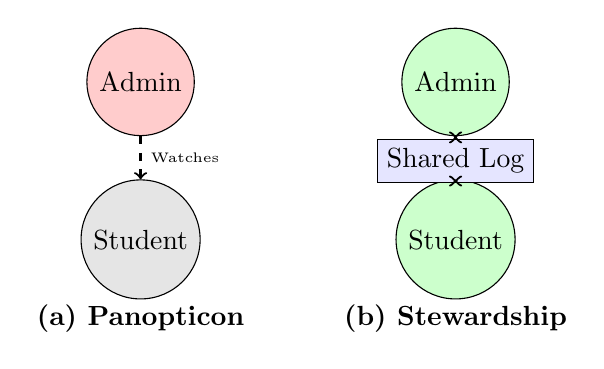
\begin{tikzpicture}
    % LEFT: ASYMMETRY
    \node (Admin1) [circle, draw, fill=red!20] at (0,2) {Admin};
    \node (Student1) [circle, draw, fill=gray!20] at (0,0) {Student};
    \draw[->, thick, dashed] (Admin1) -- node[right, font=\tiny] {Watches} (Student1);
    \node at (0,-1) {\textbf{(a) Panopticon}};

    % RIGHT: SYMMETRY
    \node (Admin2) [circle, draw, fill=green!20] at (4,2) {Admin};
    \node (Student2) [circle, draw, fill=green!20] at (4,0) {Student};
    \node (System) [rectangle, draw, fill=blue!10] at (4,1) {Shared Log};
    \draw[<->, thick] (Admin2) -- (System);
    \draw[<->, thick] (Student2) -- (System);
    \node at (4,-1) {\textbf{(b) Stewardship}};
\end{tikzpicture}
\caption{Information Asymmetry vs. Symmetry. In (a), only the Admin sees. In (b), both parties audit a shared ledger, establishing trust.}
\label{fig:symmetry}
\end{figure}

\subsection{Algorithmic Fairness and Bias Perception}
A major component of trust is the perception of fairness. Benjamin \cite{b15} and Noble \cite{b16} have documented how automated systems often encode racial and gender biases. In our study, minority students initially expressed higher skepticism (Phase 1). However, participants reported perceiving the skeleton representation as less susceptible to identity-based discrimination. By showing that the system visibly tracks geometry ($x,y,z$ coordinates) rather than skin texture or cultural markers, it alleviated fears of discriminatory profiling. This aligns with Mitchell et al.'s \cite{b17} call for transparent reporting.

\subsection{Jurisdictional Variance \& Legal Harmonization}
While this study references the General Data Protection Regulation (GDPR) \cite{b26} as a gold standard for privacy expectations, interpretations vary globally. In the Indian context, under the \textit{Digital Personal Data Protection (DPDP) Act 2023}, the emphasis shifts towards the role of the ``Data Fiduciary.'' Systems designed around volatile memory processing avoid complex multi-jurisdictional data retention liabilities, as no persistent raw biometric data is created, lowering the psychological barrier for institutional adoption.

\subsection{The Role of Explainability}
While previous evaluations established that context-aware fusion improves algorithmic accuracy, this study evaluated its impact strictly on sociological trust perception. Advanced logic is initially viewed with suspicion (``Why did my engagement score drop? Is the AI biased?''). When the \textbf{Inference Logic} was exposed via the Audit App (``Score dropped because `Head Down' detected for >2 minutes''), student complaints dropped substantially. Explainability transforms the system from an arbitrary, opaque judge to a helpful, transparent coach.

\subsection{Mitigating the Chilling Effect}
Surveillance literature often cites the ``Chilling Effect''---the inhibition of legitimate behavior due to the fear of observation. In Phase 1, we observed signs of this: students in the back rows sat rigidly, fearing that slouching would be penalized. In Phase 2, informal classroom observations suggested a reduction in visible posture rigidity. The ``Skeleton View'' acted as a visual contract, proving that posture was monitored but identity was not linked to micro-behaviors. 

\subsection{The Paradox of Transparency}
We observed a minor negative effect: ``Information Overload.'' Initially, the Audit App showed raw JSON logs, which confused some students. We iterated to show simplified summaries (e.g., ``Attendance: Present''). This highlights that transparency must be \textbf{curated}. Dumping raw data can decrease trust if it increases confusion. The ``Glass Box'' must be a clean window, not a cluttered one.

\subsection{Institutional Implications}
Administrators initially feared that transparency would lead to ``gaming the system''---that students would learn to trick the AI. The study found the opposite: transparency led to \textbf{cooperation}. Students stopped trying to hide from cameras once they understood the cameras were not recording faces. By treating students as partners rather than targets, the system fostered a cooperative security culture.

% ==========================================
% VII. CONCLUSION
% ==========================================
\section{Conclusion}
This longitudinal study demonstrates a strong association between visible transparency interventions and increased perceived trust, suggesting that the ``Big Brother'' effect is not an inevitable consequence of AI monitoring, but a design failure of opaque architectures. By exposing the inner workings of the system to the subjects being monitored, we transformed student perception from fear to trust ($2.4 \to 4.1$).

The key sociological finding is that \textbf{user experience design plays a decisive mediating role between architectural privacy properties and perceived trust}. Advanced cryptographic or statistical privacy controls are necessary foundations, but they are insufficient for social acceptance because they are invisible. Users must be able to *see* the privacy boundaries to believe in them. The visual abstraction interfaces provided this visibility, acting as tangible proof of privacy. 

While the results indicate strong association, the study design does not isolate transparency as the sole causal factor. Temporal familiarity and novelty effects cannot be fully ruled out. Nevertheless, we conclude that future academic AI systems must treat \textbf{Explainability and Visibility} as first-class functional requirements, equal in importance to Accuracy and Latency. ``Automated Stewardship'' is achievable, but only if the system is designed to be seen as clearly as it sees.

% ==========================================
% REFERENCES
% ==========================================
\begin{thebibliography}{00}

\bibitem{b25} L. J. Cronbach, ``Coefficient alpha and the internal structure of tests,'' \textit{Psychometrika}, vol. 16, no. 3, pp. 297--334, 1951.

\bibitem{b1} J. Bentham, \textit{The Panopticon Writings}. Verso, 1995.

\bibitem{b6} R. C. Mayer, J. H. Davis, and F. D. Schoorman, ``An integrative model of organizational trust,'' \textit{Academy of Management Review}, 1995.

\bibitem{b5} J. D. Lee and K. A. See, ``Trust in automation: Designing for appropriate reliance,'' \textit{Human Factors}, 2004.

\bibitem{b2} D. J. Solove, ``A Taxonomy of Privacy,'' \textit{University of Pennsylvania Law Review}, 2006.

\bibitem{b13} A. Cavoukian, ``Privacy by Design: The 7 Foundational Principles,'' \textit{Information and Privacy Commissioner of Ontario}, 2009.

\bibitem{b4} H. Nissenbaum, \textit{Privacy in Context: Technology, Policy, and the Integrity of Social Life}. Stanford University Press, 2009.

\bibitem{b11} S. Slade and P. Prinsloo, ``Learning analytics: Ethical issues and dilemmas,'' \textit{American Behavioral Scientist}, vol. 57, no. 10, pp. 1510-1529, 2013.

\bibitem{b8} K. Crawford and J. Schultz, ``Big data and due process: Toward a framework to redress predictive privacy harms,'' \textit{Boston College Law Review}, 2014.

\bibitem{b14} F. Pasquale, \textit{The Black Box Society: The Secret Algorithms That Control Money and Information}. Harvard University Press, 2015.

\bibitem{b9} M. Hildebrandt, ``Smart technologies and the end(s) of law,'' \textit{Edward Elgar Publishing}, 2015.

% --- EXPANDED REFERENCES ---

\bibitem{b22} K. O'Neil, \textit{Weapons of Math Destruction}. Crown, 2016.

\bibitem{b26} European Parliament and Council of the European Union, ``Regulation (EU) 2016/679 (General Data Protection Regulation),'' \textit{Official Journal of the European Union}, 2016.

\bibitem{b7} J. Penney, ``Chilling Effects: Online Surveillance and Wikipedia Use,'' \textit{Berkeley Technology Law Journal}, vol. 31, no. 1, 2016.

\bibitem{b12} B. Williamson, ``Big Data in Education: The Digital Future of Learning, Policy and Practice,'' \textit{Sage}, 2017.

\bibitem{b24} J. Cheney-Lippold, \textit{We Are Data: Algorithms and the Making of Our Digital Selves}. NYU Press, 2017.

\bibitem{b3} S. Kokolakis, ``Privacy attitudes and privacy behaviour: A review of current research on the privacy paradox phenomenon,'' \textit{Computers \& Security}, vol. 64, pp. 122--134, 2017.

\bibitem{b16} S. U. Noble, \textit{Algorithms of Oppression: How Search Engines Reinforce Racism}. NYU Press, 2018.

\bibitem{b19} D. Beer, ``The data gaze: Capitalism, power and perception,'' \textit{Sage}, 2018.

\bibitem{b23} V. Eubanks, \textit{Automating Inequality}. St. Martin's Press, 2018.

\bibitem{b10} S. Zuboff, \textit{The Age of Surveillance Capitalism}. PublicAffairs, 2019.

\bibitem{b15} R. Benjamin, \textit{Race After Technology: Abolitionist Tools for the New Jim Code}. Polity, 2019.

\bibitem{b17} M. Mitchell et al., ``Model Cards for Model Reporting,'' \textit{FAT* '19}, 2019.

\bibitem{b18} N. Couldry and U. A. Mejias, ``Data Colonialism: Rethinking Big Data's Relation to the Contemporary Subject,'' \textit{Television \& New Media}, 2019.

\bibitem{b20} S. Andrejevic, ``Automated Media,'' \textit{Routledge}, 2019.

\bibitem{b21} L. Amoore, ``Cloud Ethics: Algorithms and the Attributes of Ourselves and Others,'' \textit{Duke University Press}, 2020.

\bibitem{scholarmaster_repo} Narendra Babu P, ``ScholarMasterEngine,'' 2025. [Online]. Available: \url{https://github.com/NarendraaP/ScholarMasterEngine}.

\end{thebibliography}

\end{document}